\documentclass[journal]{IEEEtran}
\usepackage[a5paper, margin=10mm, onecolumn]{geometry}
\usepackage{amsmath,amssymb,amsfonts,amsthm}
\usepackage{mathtools}
\usepackage{gvv-book}
\usepackage{gvv}
\usepackage{hyperref}

\begin{document}

\title{5.8.43}
\author{Puni Aditya - EE25BTECH11046}
\maketitle

\textbf{Question:}

The sum of three numbers is 6. If we multiply the third number by 3 and add the second number to it, we get 11. By adding the first and third numbers, we get double of the second number. Find the numbers.

\textbf{Solution:}
Given
\begin{align}
    x+y+z &= 6 \\
    0x+y+3z &= 11 \\
    x-2y+z &= 0
\end{align}
\begin{align}
    \myaugvec{3}{
        1 & 1 & 1 & 6 \\
        0 & 1 & 3 & 11 \\
        1 & -2 & 1 & 0
    }
    \xleftrightarrow{\text{R}_3 \to \text{R}_3 - \text{R}_1}
    \myaugvec{3}{
        1 & 1 & 1 & 6 \\
        0 & 1 & 3 & 11 \\
        0 & -3 & 0 & -6
    }
\end{align}
\begin{align}
    \xleftrightarrow{\text{R}_3 \to -\frac{1}{3}\text{R}_3}
    \myaugvec{3}{
        1 & 1 & 1 & 6 \\
        0 & 1 & 3 & 11 \\
        0 & 1 & 0 & 2
    }
    \xleftrightarrow{\text{R}_2 \leftrightarrow \text{R}_3}
    \myaugvec{3}{
        1 & 1 & 1 & 6 \\
        0 & 1 & 0 & 2 \\
        0 & 1 & 3 & 11
    }
\end{align}
\begin{align}
    \xleftrightarrow[\text{R}_3 \to \text{R}_3 - \text{R}_2]{\text{R}_1 \to \text{R}_1 - \text{R}_2}
    \myaugvec{3}{
        1 & 0 & 1 & 4 \\
        0 & 1 & 0 & 2 \\
        0 & 0 & 3 & 9
    }
    \xleftrightarrow{\text{R}_3 \to \frac{1}{3}\text{R}_3}
    \myaugvec{3}{
        1 & 0 & 1 & 4 \\
        0 & 1 & 0 & 2 \\
        0 & 0 & 1 & 3
    }
\end{align}
\begin{align}
    \xleftrightarrow{\text{R}_1 \to \text{R}_1 - \text{R}_3}
    \myaugvec{3}{
        1 & 0 & 0 & 1 \\
        0 & 1 & 0 & 2 \\
        0 & 0 & 1 & 3
    }
\end{align}
\begin{align*}
    \myvec{x \\ y \\ z} = \myvec{1 \\ 2 \\ 3}
\end{align*}
$\therefore$ The required numbers are 1,2 and 3.

\begin{figure}[h!]
	\centering
	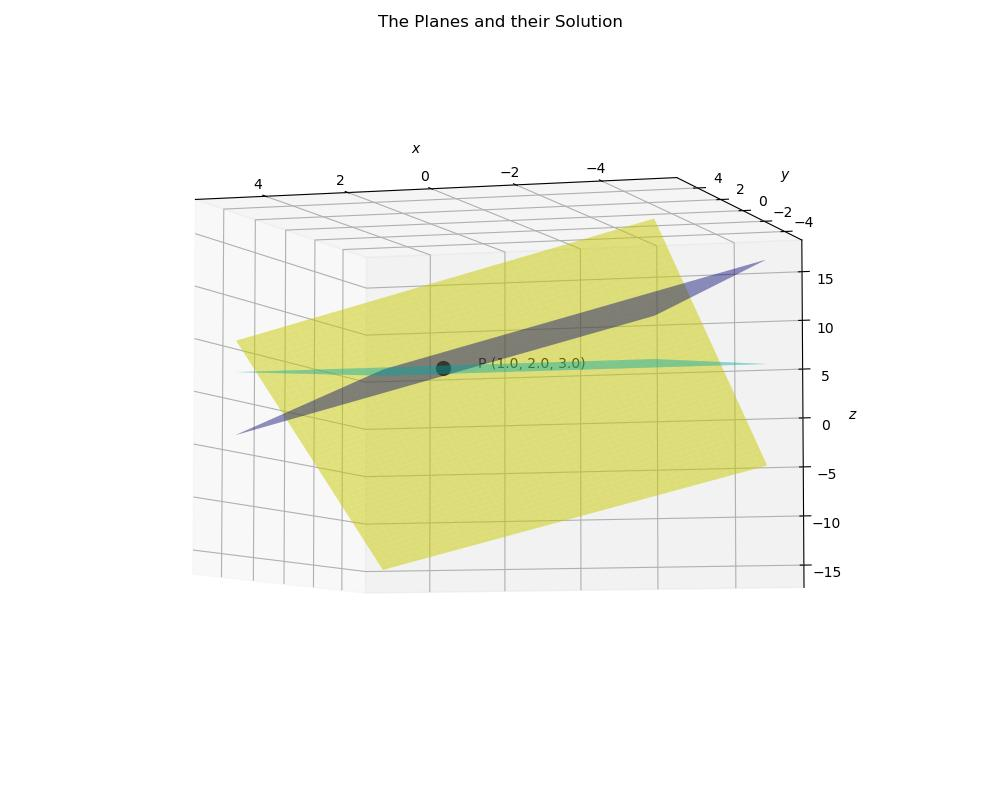
\includegraphics[width=\columnwidth]{figs/plot_c.jpg}
	\caption*{Plot}
	\label{fig:fig}
\end{figure}

\end{document}
